\documentclass[10pt,twocolumn,letterpaper]{article}

\usepackage{cvpr}
\usepackage{times}
\usepackage{epsfig}
\usepackage{graphicx}
\usepackage{amsmath}
\usepackage{amssymb}
\usepackage{graphicx} % Allows you to include images
\usepackage{hyperref}
\usepackage{enumitem} % Allows customization of list spacing
\usepackage{float} % To control float positioning
\usepackage{placeins} % For FloatBarrier

% Include other packages here, before hyperref.

% If you comment hyperref and then uncomment it, you should delete
% egpaper.aux before re-running latex.  (Or just hit 'q' on the first latex
% run, let it finish, and you should be clear).
\usepackage[pagebackref=true,breaklinks=true,letterpaper=true,colorlinks,bookmarks=false]{hyperref}

\cvprfinalcopy % *** Uncomment this line for the final submission

\def\cvprPaperID{****} % *** Enter the CVPR Paper ID here
\def\httilde{\mbox{\tt\raisebox{-.5ex}{\symbol{126}}}}

% Pages are numbered in submission mode, and unnumbered in camera-ready
%\ifcvprfinal\pagestyle{empty}\fi
\begin{document}

%%%%%%%%% TITLE
\title{Project Report : CS 7643}

\author{Girish Sharma\\
{\tt\small gsharma@gatech.edu}
% For a paper whose authors are all at the same institution,
% omit the following lines up until the closing ``}''.
% Additional authors and addresses can be added with ``\and'',
% just like the second author.
% To save space, use either the email address or home page, not both
\and
Matias Vizcaino \\
{\tt\small avizcaino3@gatech.edu}
\and
William Gleason\\
{\tt\small wgleason3@gatech.edu}
}

\maketitle
%\thispagestyle{empty}

%%%%%%%%% ABSTRACT
\begin{abstract}
   In this paper, we evaluate adapters as a parameter efficient alternative to fine-tuning a model for a given task. We first fine-tune a pre-trained model to perform a given task and then use the same pre-trained model to introduce adapter modules and perform the same task using an adapter-based approach. We see that adapters can achieve comparable performance to fine-tuning. But adapters also have significant benefits over fine-tuning, in terms of greatly reduced trainable parameters, ability to perform sequential training on tasks, and combining multiple adapters to create a single model capable of performing multiple tasks.
\end{abstract}

%%%%%%%%% BODY TEXT
\section{Introduction/Background/Motivation}

\subsection{Objective} We aimed to understand how traditional methods using fine-tuning compare to newer architectures using adapters in the context of pre-trained models for natural language processing. We conducted this comparison across 4 types of pre-trained models that have been used before in other studies \cite{gururangan2020dont}. 1. A generic LLM, RoBERTa. 2. An LLM pre-trained on text in the domain of a task (DAPT). 3. An LLM pre-trained on the unlabeled data from a specific task (TAPT) 4. LLM pre-trained on both (DAPT + TAPT). 

We also experimented with different adapter configurations to understand how they achieve parameter-efficient transfer learning and if there are any trade-offs between different architectures.

Additionally, we evaluate the effectiveness of a new architecture that leverages multiple adapters using an attention layer called Adapter Fusion. We evaluated the impact of the adapter architectures by the F1-Macro Score and the reduction in the number of trainable parameters.

\subsection{Current State} A common practice today is to start with a model pre-trained on a broad corpus of information and then use fine-tuning to train the model for a particular task. To achieve this, we first add any task specific heads as the final layers to the pre-trained model. We then co-train the pre-trained weights and a new top-layer with task specific labeled data. Fine-tuning has been shown to be a very effective at performing a given task.
\begin{itemize}
\item \textbf{Full Fine-Tuning} One option is to retrain the entire model on the task data. While this would likely lead to the best performance, studies have shown that this full fine-tuning is often unnecessary. Earlier layers of the pre-trained model generally learn broad semantic and syntactic features and those don’t really change for any given task. 
\item \textbf{Variable Fine-Tuning} A more efficient way to fine-tune is to selectively modify the weights of n layers of the model, of the pre-trained model, keeping the earlier layers frozen. We then retrain this updated model with the task data. The resultant performance has been shown to be similar to full fine-tuning \cite{houlsby2019parameter}, but with reduced trainable parameters.
\item \textbf{Continued Pre-Training} Rather than directly fine-tuning, the model first undergoes additional pre-training via Domain Adaptive Pre-Training (DAPT) or Task Adaptive Pre-Training (TAPT). The model becomes more familiar with the types of texts and context it will encounter in the task. This pre-adaptation helps in dealing with domain-specific language challenges and make the most out of available data in both unlabeled and labeled forms \cite{gururangan2020dont}.
\end{itemize}
\subsection{Motivation}  Fine-tuning has several drawbacks.
\begin{itemize}
    \item Fine-tuning involves training a large number of parameters for each task. For large models which can be 100s of MB, storing and sharing a complete set of weights for each task can limit multi-task applications.
    \item All tasks must be trained simultaneously. Sequential fine-tuning for multiple tasks leads to catastrophic forgetting \cite{mccloskey1989catastrophic}
\end{itemize}
Adapters do not suffer from these drawbacks \cite{houlsby2019parameter}. The number of trained parameters is a tiny fraction compared to fine-tuning, significantly reducing the computational resources for fine-tuning \ref{tab:model-parameters}. Additionally, adapters are modular as they can be loaded onto the same base model to perform multiple tasks, eliminating the need for a copy of the base model for each task. Further, as they preserve the original model weights, they are more capable of preserving the base model integrity and performance across tasks.

Studies, like those by Gururangan et al. \cite{gururangan2020dont} highlight the benefits of domain-adaptive pre-training (DAPT) and task-adaptive pre-training (TAPT), which tailor the pre-training phase to more closely align with the characteristics of the target tasks, potentially enhancing subsequent fine-tuning outcomes. While these studies primarily focus on the impacts of adapting pre-training in low-vocabulary overlap tasks, their insights are crucial for informing more efficient strategies where only a fraction of the model’s parameters are adjusted to achieve task-specific tuning. In “Parameter-Efficient Transfer Learning for NLP” \cite{houlsby2019parameter}, the authors show that adapters attain within 0.4\% of the performance of full-fine-tuning, adding only 3.6\% parameters per task. The paper used the BERT transformer as its pre-trained model and used tasks from the GLUE benchmark to prove its assertions. We will be using the RoBERTa model, which is a more robust version of BERT \cite{liu2019roberta}.

\begin{table*}[t]
  \centering
  
  \begin{tabular}{ l l l r r r r }
    \hline
    \textbf{Domain} & \textbf{Task} & \textbf{Label Type} & \textbf{Train} & \textbf{Dev}   & \textbf{Test}  & \textbf{Classes} \\
    \hline
    Computer Science & ACL-ARC & citation intent & 1,688 & 114   & 139   & 6 \\
                     & SCIERC  & relation classification & 3,219 & 455   & 974   & 7 \\
    \hline
    BIOMED           & CHEMPROT & relation classification & 4,169 & 2,427 & 3,469 & 13 \\
    \hline
  \end{tabular}%
  \caption{\textbf{Dataset Statistics}}
  \label{tab:dataset-stats}%
\end{table*}%

\begin{table*}[htbp]
    \centering
    
    \begin{tabular}{ l r r r }
        \hline
        \textbf{Model} & \textbf{Parameter Counts} & \textbf{Parameters Trained} & \textbf{Percentage Trained} \\
        \hline
        RoBERTa & 124,650,246 & 124,650,246 & 100.00\% \\
        Pfeiffer Adapters & 126,777,759 & 2,127,513 & 1.71\% \\
        Houlsby Adapters & 127,672,287 & 3,022,041 & 2.42\% \\
        \hline
    \end{tabular}
    \caption{\textbf{Model Parameters and Training Percentage}}
    \label{tab:model-parameters}
\end{table*}

\subsection{Data, Domain, and Tasks} The tasks (used in earlier studies\cite{gururangan2020dont}) we primarily focus on are under the CS domain, ACL-ARC (citation-intent) and SCIERC (relation classification) . We further add one task from BIOMED domain, CHEMPROT (relation classification) \footnote{Attempts were made to train on high-resource tasks, but due to computational demands, this was infeasible within our timeframe and is set as a future objective. We further exclude the low-resource NEWS task HYPERPARTISIAN as the test/validation dataset is very small and has only 2 classes - this leads to inconsistent results from \cite{allenai_dont_stop_pretraining} under our current set-up, again to be investigated as a future objective.}, to test the hypothesis under a new domain. All these tasks have under 5,000 training records (i.e., low-resource). Table \ref{tab:dataset-stats}.

The task-specific datasets are made available to download by Allen Institute \cite{allenai_dont_stop_pretraining}. We use Macro-F1 as the performance metrics, which is a harmonic mean of precision and recall. Both task datasets show similar class distribution and are imbalanced. However, since we are comparing fine-tuning with adapters, it would not affect the final comparison.

\textbf{Base Models and Fine-Tuning} For reproduction, we first aimed to use the same set-up as in the published paper \cite{allenai_dont_stop_pretraining} but encountered limitations on compatibility with newer packages and versioning. Therefore, we chose the widely used HuggingFace Transformers library \cite{transformers} and ecosystem for loading and training our models. We load the pre-trained models from HuggingFace \cite{allenai_dont_stop_pretraining} and train a classification head in supervised manner using the same task-specific datasets and approach as in the original paper \cite{gururangan2020dont}. Our replicated F1 metric is taken as a benchmark to assess the performance of adapter methods.

\textbf{Adapters}  To assess the efficacy of adapter methods, for every task we add task-specific adapters (and a prediction head) to each of the base models and train them on the task-specific data. For training and managing adapters, we use AdapterHub’s library \cite{adapterhub_overview} and two of their adapter architectures: Pfeiffer \cite{pfeiffer2020adapterhub} a lightweight configuration that adds the adapter modules between the feed-forward layers, and Houlsby \cite{houlsby2019parameter} which can handle more complexity as it adds adapter modules between the multi-head attention layer. The APPENDIX \ref{sec:pfeiffermodel} \ref{sec:houlsbymodel} shows examples of the adapter modules added to the model for both configurations. We compare results under two scopes: direct fine-tuning comparison, and second phase of pre-training comparison.


%-------------------------------------------------------------------------
%------------------------------------------------------------------------
\section{Approach}

\subsection{Methodology} Our objective is to compare fine-tuning transfer learning for a given task with an adapters-based approach. For this we recreate the baseline that was used in the transfer learning paper \cite{gururangan2020dont}. We then perform the same transfer learning by using two adapter configurations, Pfeiffer and Houlsby. We use the same evaluation metrics that were used in the original paper \cite{gururangan2020dont}. We do this for all the four pre-trained models. This should give us a comparison for transfer learning using full fine-tuning, Pfeiffer adapters, and Houlsby adapters. For all our experimentation, we use the huggingface libraries transformers \cite{transformers} and adapters \cite{adapters}.

\subsection{Outcome} Optuna was chosen as our hyperparameter optimization framework, especially useful in adapter training to traverse the combinations of learning rates, batch sizes and epochs. The framework proved useful for streamlining the hyperparameter search and selecting the next set-up that would likely lead to an improvement in the F1 performance metric, and monitoring/reporting. Each combination runs within a trial, and each trial is composed of 5 random seeds. The mean F1 is set as a performance metric, and the best and standard deviation for the best set-up on the test dataset is reported.  

\subsection{Hypothesis} Based on recent research showing the efficacy of adapters at performing on par with fine-tuning approaches \cite{houlsby2019parameter}, we felt confident that we can get comparable results with adapters. This should be enough to consider adapters as a replacement to fine-tuning, since adapters allow for a lot of flexibility with smaller number of trainable parameters, ability to stack multiple adapters onto the same model, and sequential learning on multiple tasks. Further, we were not very sure if our datasets, given their small size, would be able to highlight any differences between the Pfeiffer and Houlsby architectures. Given the higher number of trainable parameters with Houlsby configuration, we expected Houlsby to have a better performance.

\subsection{Optimization} By using Optuna for hyper-parameter optimization, we were able to create better adapter based results. We used the huggingface library transformers and adapters for our training, which use the Adam optimizer (default) with L2 regularization. Since our tasks were all related to classification, cross-entropy loss was used for training. 

\subsection{Challenges} We were not able to recreate the results of the transfer learning paper \cite{gururangan2020dont} as we used different libraries than the ones used in the paper. However, with hyper-parameter optimization using Optuna, we were able to create fine-tuning results that were as good as the reference paper (better in some cases). Hence, we compare our adapter's performance to our own fine-tuning results. The processes we ran also showed a lot of stochasticity across runs. We smoothed out most of the variance by the use of five random seeds, which helped in comparing across different runs.


\section{Experiments and Results}

For our fine-tuning experiments, we add a classifier layer to the pre-trained models and co-train all the pre-trained weights and the classifier with the task data.

For our adapters-based experiments, we add the adapters to the pre-trained models and the classification heads. We then train the adapters, which only trains the adapter layers and the final classification heads, without changing any of the pre-trained weights.


\subsection{Results}


Table \ref{tab:model-parameters} shows the total parameter counts of the models when using fine-tuning and the adapters. Note that the Pfeiffer configuration is much more parameter-efficient than the Houlsby configuration, as it introduces fewer layers. A sample of the layers can be found in the appendix \ref{sec:pfeiffermodel} \ref{sec:houlsbymodel}.


\begin{table*}[h]
\centering

\begin{tabular}{lcccc}
\hline
\textbf{Pre-trained Model} & \textbf{Baseline} & \textbf{Fine Tuning} & \textbf{Adapter Pfeiffer} & \textbf{Adapter Houlsby} \\
\hline
% ACL-ARC
\multicolumn{5}{c}{\textbf{ACL-ARC}} \\
ROBERTA & 63.00 $\pm$ 1.50 & 66.34 $\pm$ 4.67 & 67.12 $\pm$ 1.85 & 65.53 $\pm$ 1.30 \\
TAPT & 67.40 $\pm$ 1.50 & 69.49 $\pm$ 2.24 & 67.22 $\pm$ 5.09 & 65.12 $\pm$ 1.22 \\
DAPT & 75.40 $\pm$ 2.00 & 74.65 $\pm$ 1.35 & 73.32 $\pm$ 2.70 & 74.03 $\pm$ 3.96 \\
DAPT-TAPT & 75.60 $\pm$ 5.80 & 74.89 $\pm$ 2.45 & 73.20 $\pm$ 2.54 & 74.12 $\pm$ 4.85 \\
\hline
% SCIERC
\multicolumn{5}{c}{\textbf{SCIERC}} \\
ROBERTA & 77.30 $\pm$ 1.90 & 80.02 $\pm$ 1.20 & 81.60 $\pm$ 0.42 & 81.32 $\pm$ 0.71 \\
TAPT & 79.30 $\pm$ 1.10 & 80.95 $\pm$ 0.74 & 80.80 $\pm$ 1.35 & 80.92 $\pm$ 0.76 \\
DAPT & 80.80 $\pm$ 1.20 & 83.08 $\pm$ 1.16 & 82.48 $\pm$ 0.54 & 82.55 $\pm$ 0.81 \\
DAPT-TAPT & 81.30 $\pm$ 1.50 & 81.55 $\pm$ 0.74 & 81.47 $\pm$ 0.70 & 82.81 $\pm$ 0.55 \\
\hline
% CHEMPROT
\multicolumn{5}{c}{\textbf{CHEMPROT}} \\
ROBERTA & 81.90 $\pm$ 0.10 & 80.69 $\pm$ 0.55 & 80.38 $\pm$ 0.32 & 80.95 $\pm$ 0.40 \\
TAPT & 82.60 $\pm$ 0.11 & 79.88 $\pm$ 0.88 & 80.80 $\pm$ 0.35 & 80.67 $\pm$ 0.65 \\
DAPT & 84.20 $\pm$ 0.02 & 81.72 $\pm$ 0.42 & 81.85 $\pm$ 0.51 & 82.16 $\pm$ 0.68 \\
DAPT-TAPT & 84.40 $\pm$ 0.40 & 81.71 $\pm$ 0.52 & 81.67 $\pm$ 0.30 & 82.29 $\pm$ 0.40 \\
\hline
\end{tabular}
\caption{\textbf{Comparison of Fine-tuning, Pfeiffer Adapters, and Houlsby Adapters}}
\label{tab.adaptersvsftresults}
\end{table*}


\subsection{Adapters vs fine-tuning} Based on our empirical results \ref{tab.adaptersvsftresults}, we see that adapters were able to achieve similar performance as full fine-tuning. There is some variation attributable to optimal hyper-parameter settings and the limited time and resources we used to conduct these experiments. However, the results clearly demonstrate the capacity of adapters to be as effective at transfer learning as full fine-tuning. The comparison of the models \ref{tab:model-parameters} shows that the adapters needed just a fraction of the total parameters (1.71\% and 2.42\%) to be trained to achieve comparable results. While this is a very small sample set, other works have shown similar results \cite{houlsby2019parameter} with adapters and our experiments are in-line with the expectations.

\begin{table*}[h]
\centering
\begin{tabular}{lcccc}
\hline
\textbf{Dataset} & \textbf{Pre-trained Model} & \textbf{Baseline} & \textbf{Fine Tuning} & \textbf{Adapter Pfeiffer} \\
\hline
\multicolumn{6}{c}{ACL-ARC} \\
ROBERTA & 63.00 $\pm$ 1.50 & 66.34 $\pm$ 4.67 & 67.12 $\pm$ 1.85 & 65.53 $\pm$ 1.30 \\
TAPT & 67.40 $\pm$ 1.50 & 69.49 $\pm$ 2.24 & 67.22 $\pm$ 5.09 & 65.12 $\pm$ 1.22 \\
DAPT & 75.40 $\pm$ 2.00 & 74.65 $\pm$ 1.35 & 73.32 $\pm$ 2.70 & 74.03 $\pm$ 3.96 \\
DAPT-TAPT & 75.60 $\pm$ 5.80 & 74.89 $\pm$ 2.45 & 73.20 $\pm$ 2.54 & 74.12 $\pm$ 4.85 \\
\hline
\multicolumn{6}{c}{SCIERC} \\
ROBERTA & 77.30 $\pm$ 1.90 & 80.02 $\pm$ 1.20 & 81.60 $\pm$ 0.42 & 81.32 $\pm$ 0.71 \\
TAPT & 79.30 $\pm$ 1.10 & 80.95 $\pm$ 0.74 & 80.80 $\pm$ 1.35 & 80.92 $\pm$ 0.76 \\
DAPT & 80.80 $\pm$ 1.20 & 83.08 $\pm$ 1.16 & 82.48 $\pm$ 0.54 & 82.55 $\pm$ 0.81 \\
DAPT-TAPT & 81.30 $\pm$ 1.50 & 81.55 $\pm$ 0.74 & 81.47 $\pm$ 0.70 & 82.81 $\pm$ 0.55 \\
\hline
\multicolumn{6}{c}{CHEMPROT} \\
ROBERTA & 81.90 $\pm$ 0.10 & 80.69 $\pm$ 0.55 & 80.38 $\pm$ 0.32 & 80.95 $\pm$ 0.40 \\
TAPT & 82.60 $\pm$ 0.11 & 79.88 $\pm$ 0.88 & 80.80 $\pm$ 0.35 & 80.67 $\pm$ 0.65 \\
DAPT & 84.20 $\pm$ 0.02 & 81.72 $\pm$ 0.42 & 81.85 $\pm$ 0.51 & 82.16 $\pm$ 0.68 \\
DAPT-TAPT & 84.40 $\pm$ 0.40 & 81.71 $\pm$ 0.52 & 81.67 $\pm$ 0.30 & 82.29 $\pm$ 0.40 \\
\hline
\end{tabular}
\caption{\textbf{Adapters as an alternative to TAPT}}
\label{tab.taptadatperresults}
\end{table*}


\subsection{Adapters vs Continued Pre-Training} Adapters serve as both a complement to traditional fine-tuning and as a standalone alternative, offering targeted task optimization while reducing computational costs, which is especially beneficial in settings with limited resources.

In addition, we observe that adapters achieve comparable performance to traditional fine-tuning and TAPT methods in many cases \ref{tab.taptadatperresults}. This suggests they are capable of effectively transferring the knowledge from pre-trained models to specific tasks without the need to adjust all model weights. In some cases, using adapters without additional task-specific pre-training (Adapter (Base)) provided comparable performance to using TAPT, indicating that adapters can serve as an alternative to TAPT, especially when resources for additional pre-training are limited. TAPT may not provide as much benefit over adapters since the task-specific terms may not be well-represented in the pre-training corpus. Adapters, however, allow for more targeted adjustments to the model, focusing specifically on the task-relevant aspects of the language without requiring extensive re-training of the model.

The experiments suggest that domain-specific pre-training (DAPT) provides a strong foundation for tasks within that domain, and adapters can effectively leverage and build upon this foundation. Adapters appear to be effective across different sizes of datasets. For smaller datasets, like ACL-ARC and SCIERC, they can provide the necessary specialization without extensive re-training. For larger datasets, such as CHEMPROT, adapters still maintain or improve performance, indicating their utility across different scales of data availability.



\subsection{Pfeiffer vs Houlsby} Given the higher number of trainable parameters with Houlsby compared to Pfeiffer, we expected Houlsby configuration to perform better than Pfeiffer, in general. While the sample size is small to imply too broad a conclusion, we can see that for the chosen tasks and with the hyper-parameters chosen, the Houlsby configuration was slightly better than Pfeiffer, especially when the dataset is larger. When the datasets are small there is no discernible difference, as both configurations are equally capable of optimal learning. It is expected that Houlsby would be better generally, given the higher number of trained parameters introduced by the Houlsby configuration (2.42\% vs 1.71\%). However, Pfeiffer configuration does have a definite advantage of being more parameter-efficient and this would be a desirable quality when we are talking of lots of tasks. We could see a bit of tradeoff in parameter-efficient configuration vs task performance for bigger datasets.

\subsection{Adapter Composition/Fusion}
TBD


\begin{table}[h]
\centering
\begin{tabular}{lcccc}
\hline
\textbf{Task} & \textbf{Model Used} & \textbf{Fine Tuning} & \textbf{Standalone Adapter} & \textbf{Adapter Fusion} \\
\hline
ACL-ARC & RoBERTa & 66.34$ \pm$ 4.46 & 67.12 $\pm$ 1.85 & 68.46 $\pm$ 3.43 \\
 & DAPT & 74.49 $\pm$ 3.33 & 73.32 $\pm$ 1.79 & 70.36 $\pm$ 1.87 \\
 \hline
SCIERC & RoBERTa & 80.02 $\pm$ 1.20 & 81.60 $\pm$ 0.42 & 79.84 $\pm$ 0.26 \\
 & DAPT & 83.08 $\pm$ 1.16 & 82.48 $\pm$ 0.05 & 81.32 $\pm$ 0.46 \\
\hline
\end{tabular}
\caption{\textbf{Stand-alone adapters vs Adapter Fusion}}
\label{tab:fusionresults}
\end{table}



\section{Conclusions}
Through our experiments, we were able to demonstrate the capabilities of adapters to perform at par with fine-tuning alternatives for transfer learning tasks. While needing less than 3\% of the total trainable parameters as compared to fine-tuning, the adapters performance for the tasks matched full fine-tuning.

We also see that the benefits of pre-training across domain and task applied to adapters as well.
Additionally, we also were able to compare the two popular adapter architectures – Pfeiffer and Houlsby. While the Houlsby architecture performed slightly better than the Pfeiffer architecture for our tasks and settings, Pfeiffer architecture was more parameter-efficient and comparable to Houlsby. 

Adapter composition allowed us to create a single model capable of performing multiple tasks using the parameter-efficient adapters. The combined model was at par with the individual adapters for each task since adapters do not suffer from forgetting previous tasks when learning new ones. This has significant benefits for inference, where the same model can perform multiple tasks as well as individual models, while requiring a much smaller size.

Future work could explore additional adapter architectures, composition strategies, and their application across a wider range of NLP tasks and domains.


%-------------------------------------------------------------------------
\onecolumn

\section{Team Members}




Our team was made up of three members. We all participated in periodic zoom calls where we discussed the technical details and work allocation of the project with equal participation from all.

\begin{itemize}
    \item Girish Sharma worked on the initial experiments on fine-tuning and adapters, and later worked on different adapter configurations.
    \item Matias Vizcaino worked on the implementation of the fine-tuning and adapter modules using Optuna on the PACE computers. He also studied the potential of adapters as an alternative to TAPT.
    \item William Gleason worked on the adapter composition and fusion experiments
\end{itemize}

\begin{table*}[h]
\begin{center}
\begin{tabular}{|l|c|p{8cm}|}
\hline
\textbf{Student Name} & \textbf{Contributed Aspects} & \textbf{Details} \\
\hline
Girish Sharma & Implementation and Analysis & Initial fine-tuning and adapter experiments with 5 seeds. Used manual hyper-parameter optimization. Comparison of Pfeiffer and Houlsby adapter architectures.  \\
Matias Vizcaino & Implementation and Analysis & Using Optuna-based hyper-parameter optimization for fine-tuning and adapter experiments. Created final results for fine-tuning and adapters. \\
William Gleason & Implementation and Analysis & Study of adapter composition using Adapter Fusion and other techniques. \\
\hline
\end{tabular}
\end{center}
\caption{\textbf{Contributions of team members.}}
\label{tab:contributions}
\end{table*}
\FloatBarrier


\section{Appendix}
\subsection{Task Dataset Balance}
% Insert a figure that spans both columns
\begin{figure*}[h] % 'h' suggests the figure appears in the specified location
    \centering % Center the image
    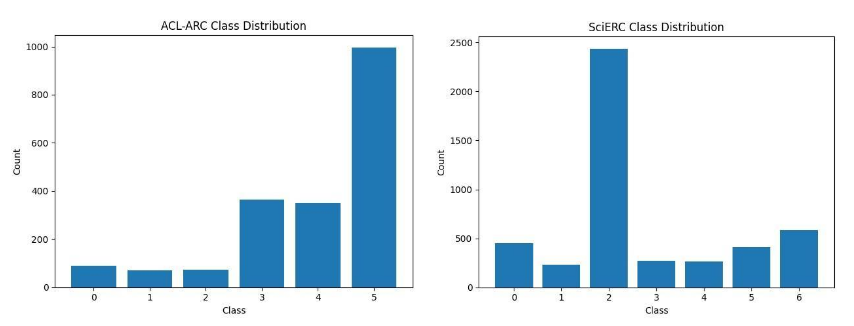
\includegraphics[width=\textwidth]{DatasetBalance.png} % Make the image full page width
    \caption{Class Distribution for ACL-ARC and SciERC datasets} % Add a caption
    \label{fig:example} % Label the figure for cross-referencing
\end{figure*}
Showing the class distribution for the two tasks in the computer science domain. \ref{fig:example}
\FloatBarrier

\subsection{Model layers}
Layers shown with parameter counts. Only showing the 1st layer for sample purposes. RoBERTa has 11 repeating layers.
\subsubsection{RoBERTa }
\label{sec:robertamodel} 
\textbf{Repeating layers}

roberta.embeddings.LayerNorm.bias: 768

roberta.encoder.layer.0.attention.self.query.weight: 589824

roberta.encoder.layer.0.attention.self.query.bias: 768

roberta.encoder.layer.0.attention.self.key.weight: 589824

roberta.encoder.layer.0.attention.self.key.bias: 768

roberta.encoder.layer.0.attention.self.value.weight: 589824

roberta.encoder.layer.0.attention.self.value.bias: 768

roberta.encoder.layer.0.attention.output.dense.weight: 589824

roberta.encoder.layer.0.attention.output.dense.bias: 768

roberta.encoder.layer.0.attention.output.LayerNorm.weight: 768

roberta.encoder.layer.0.attention.output.LayerNorm.bias: 768

roberta.encoder.layer.0.intermediate.dense.weight: 2359296

roberta.encoder.layer.0.intermediate.dense.bias: 3072

roberta.encoder.layer.0.output.dense.weight: 2359296

roberta.encoder.layer.0.output.dense.bias: 768

roberta.encoder.layer.0.output.LayerNorm.weight: 768

roberta.encoder.layer.0.output.LayerNorm.bias: 768

roberta.encoder.layer.1.attention.self.query.weight: 589824


\textbf{Final Layer}

roberta.encoder.layer.11.output.LayerNorm.bias: 768

classifier.dense.weight: 589824

classifier.dense.bias: 768

classifier.out\_proj.weight: 4608

classifier.out\_proj.bias: 6

\subsubsection{Pfeiffer Adapter}
\label{sec:pfeiffermodel} 
\textbf{Repeating layers}

roberta.embeddings.LayerNorm.bias: 768

roberta.encoder.layer.0.attention.self.query.weight: 589824

roberta.encoder.layer.0.attention.self.query.bias: 768

roberta.encoder.layer.0.attention.self.key.weight: 589824

roberta.encoder.layer.0.attention.self.key.bias: 768

roberta.encoder.layer.0.attention.self.value.weight: 589824

roberta.encoder.layer.0.attention.self.value.bias: 768

roberta.encoder.layer.0.attention.output.dense.weight: 589824

roberta.encoder.layer.0.attention.output.dense.bias: 768

roberta.encoder.layer.0.attention.output.LayerNorm.weight: 768

roberta.encoder.layer.0.attention.output.LayerNorm.bias: 768

roberta.encoder.layer.0.intermediate.dense.weight: 2359296

roberta.encoder.layer.0.intermediate.dense.bias: 3072

roberta.encoder.layer.0.output.dense.weight: 2359296

roberta.encoder.layer.0.output.dense.bias: 768

roberta.encoder.layer.0.output.LayerNorm.weight: 768

roberta.encoder.layer.0.output.LayerNorm.bias: 768

\textbf{roberta.encoder.layer.0.output.adapters.base\_citation\_intent.adapter\_down.0.weight: 36864}

\textbf{roberta.encoder.layer.0.output.adapters.base\_citation\_intent.adapter\_down.0.bias: 48}

\textbf{roberta.encoder.layer.0.output.adapters.base\_citation\_intent.adapter\_up.weight: 36864}

\textbf{roberta.encoder.layer.0.output.adapters.base\_citation\_intent.adapter\_up.bias: 768}

roberta.encoder.layer.1.attention.self.query.weight: 589824

\textbf{Final Layer}

roberta.encoder.layer.11.output.adapters.base\_citation\_intent.adapter\_up.bias: 768

roberta.pooler.dense.weight: 589824

roberta.pooler.dense.bias: 768

\textbf{heads.default.0.weight: 589824}

\textbf{heads.default.0.bias: 768}

\textbf{heads.default.2.weight: 768}

\textbf{heads.default.2.bias: 768}

\textbf{heads.default.3.bias: 50265}

\textbf{heads.base\_citation\_intent.1.weight: 589824}

\textbf{heads.base\_citation\_intent.1.bias: 768}

\textbf{heads.base\_citation\_intent.4.weight: 4608}

\textbf{heads.base\_citation\_intent.4.bias: 6}

\subsubsection{Houlsby Adapter}
\label{sec:houlsbymodel} 

\textbf{Repeating layers}

roberta.embeddings.LayerNorm.bias: 768

roberta.encoder.layer.0.attention.self.query.weight: 589824

roberta.encoder.layer.0.attention.self.query.bias: 768

roberta.encoder.layer.0.attention.self.key.weight: 589824

roberta.encoder.layer.0.attention.self.key.bias: 768

roberta.encoder.layer.0.attention.self.value.weight: 589824

roberta.encoder.layer.0.attention.self.value.bias: 768

roberta.encoder.layer.0.attention.output.dense.weight: 589824

roberta.encoder.layer.0.attention.output.dense.bias: 768

roberta.encoder.layer.0.attention.output.LayerNorm.weight: 768

roberta.encoder.layer.0.attention.output.LayerNorm.bias: 768

\textbf{roberta.encoder.layer.0.attention.output.adapters.base\_citation\_intent.adapter\_down.0.weight: 36864}

\textbf{roberta.encoder.layer.0.attention.output.adapters.base\_citation\_intent.adapter\_down.0.bias: 48}

\textbf{roberta.encoder.layer.0.attention.output.adapters.base\_citation\_intent.adapter\_up.weight: 36864}

\textbf{roberta.encoder.layer.0.attention.output.adapters.base\_citation\_intent.adapter\_up.bias: 768}

roberta.encoder.layer.0.intermediate.dense.weight: 2359296

roberta.encoder.layer.0.intermediate.dense.bias: 3072

roberta.encoder.layer.0.output.dense.weight: 2359296

roberta.encoder.layer.0.output.dense.bias: 768

roberta.encoder.layer.0.output.LayerNorm.weight: 768

roberta.encoder.layer.0.output.LayerNorm.bias: 768

\textbf{roberta.encoder.layer.0.output.adapters.base\_citation\_intent.adapter\_down.0.weight: 36864}

\textbf{roberta.encoder.layer.0.output.adapters.base\_citation\_intent.adapter\_down.0.bias: 48}

\textbf{roberta.encoder.layer.0.output.adapters.base\_citation\_intent.adapter\_up.weight: 36864}

\textbf{roberta.encoder.layer.0.output.adapters.base\_citation\_intent.adapter\_up.bias: 768}

roberta.encoder.layer.1.attention.self.query.weight: 589824

\textbf{Final Layer}

roberta.encoder.layer.11.output.adapters.base\_citation\_intent.adapter\_up.bias: 768

roberta.pooler.dense.weight: 589824

roberta.pooler.dense.bias: 768

\textbf{heads.default.0.weight: 589824}

\textbf{heads.default.0.bias: 768}

\textbf{heads.default.2.weight: 768}

\textbf{heads.default.2.bias: 768}

\textbf{heads.default.3.bias: 50265}

\textbf{heads.base\_citation\_intent.1.weight: 589824}

\textbf{heads.base\_citation\_intent.1.bias: 768}

\textbf{heads.base\_citation\_intent.4.weight: 4608}

\textbf{heads.base\_citation\_intent.4.bias: 6}

\subsection{Models}
The list below shows the pre-trained models used for the two tasks.

task\_models = \{

    \textbf{"citation\_intent"}: \{
    
        "base": "roberta-base",
        
        "dapt": "allenai/cs\_roberta\_base",
        
        "tapt":         "allenai/dsp\_roberta\_base\_tapt\_citation\_intent\_1688",
        
        "dapt\_tapt": allenai/dsp\_roberta\_base\_dapt\_cs\_tapt\_citation\_intent\_1688"
        
    \},

    \textbf{"sciie"}: \{
    
        "base": "roberta-base",
        
        "dapt": "allenai/cs\_roberta\_base",
        
        "tapt": "allenai/dsp\_roberta\_base\_tapt\_sciie\_3219",
        "dapt\_tapt": 
        "allenai/dsp\_roberta\_base\_dapt\_cs\_tapt\_sciie\_3219"
        
    \}
    
\textbf{"chemprot"}: \{

        "base": "roberta-base",
        
        "dapt": " allenai/biomed\_roberta\_base ",
        
        "tapt": " allenai/dsp\_roberta\_base\_tapt\_chemprot\_4169",
        "dapt\_tapt": " 
        allenai/dsp\_roberta\_base\_dapt\_biomed\_tapt\_chemprot\_4169"
        
    \}
    


\section{Source Code}
Source code can be found at the following link:
\href{https://github.gatech.edu/avizcaino3/CS-7643-EfficiencyLane.git}{https://github.gatech.edu/avizcaino3/CS-7643-EfficiencyLane.git}

{\small
\bibliographystyle{ieeetr}
\bibliography{references}
}

\end{document}
